% Pictures of the method and of the main result (appendix of the 9-page version).
\section{The method and the main result in pictures}
\label{app:pictures}

Figure~\ref{fig:overview} sets FK-LoRA beside one shared adapter and beside the two published
methods we ran, and Figure~\ref{fig:switch} shows the three rules that set the route. The other
figures show the runs without definitions of Section~\ref{sec:nodeftrained}:
Figure~\ref{fig:answergrid} the changed answers one by one, Figure~\ref{fig:stageheat} the score of
every task after every stage, Figure~\ref{fig:learnkeep} the runs with and without definitions side
by side, and Figure~\ref{fig:routematrix} where the test inputs of the fifteen tasks are sent after
the last task.

\begin{figure}[t]
  \centering
  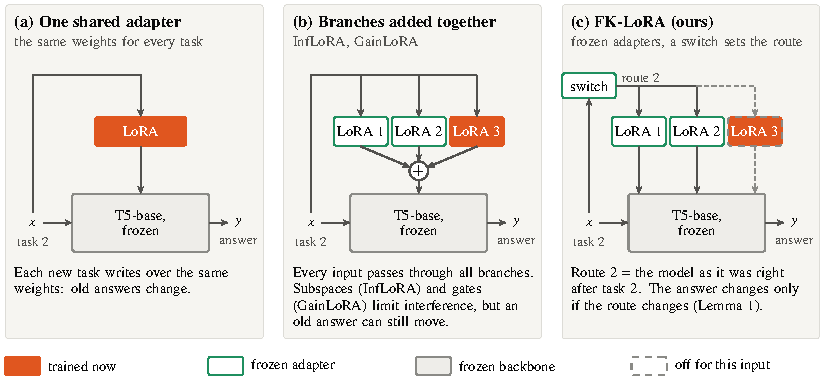
\includegraphics[width=\linewidth]{figures/overview}
  \caption{Three ways to add a task, shown while task~3 is being learned and an input of task~2 is
  answered. (a)~One shared adapter is trained again for each task, so old answers change.
  (b)~InfLoRA and GainLoRA add one branch per task, and every input passes through all branches
  (weighted by gates in GainLoRA); a chosen subspace or the gates limit what a new branch does to
  old inputs, but an old answer can still change. (c)~FK-LoRA never changes an adapter after its
  task has been learned, and a switch sets the route of each input: route~2 is the model as it was
  right after task~2, so the answer changes only if the route changes (Lemma~\ref{lem:route}).}
  \label{fig:overview}
\end{figure}

\begin{figure}[t]
  \centering
  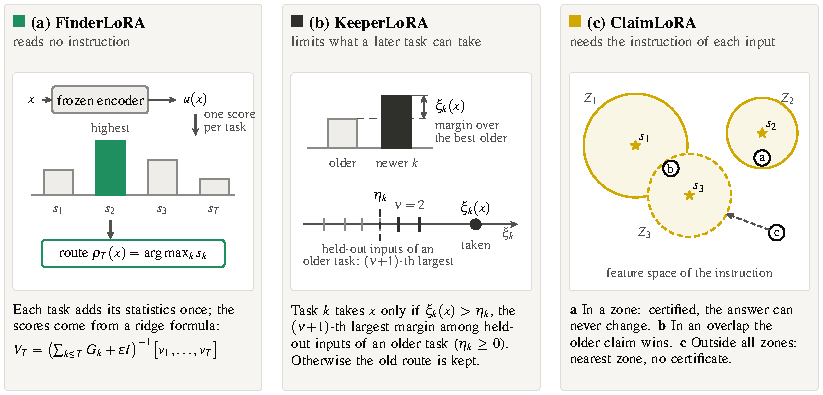
\includegraphics[width=\linewidth]{figures/switch}
  \caption{The three rules that set the route. (a)~\recog{} reads no instruction: it scores every
  task on a frozen feature $u(x)$ of the input with one ridge formula and takes the highest score.
  (b)~\handicap{} adds a handicap for a new task: task $k$ takes an input only if its margin
  $\xi_k(x)$ over the best older task is above $\eta_k$, the $(\nu+1)$-th largest margin among the
  held-out inputs of an older task ($\nu = 2$ in our runs). (c)~\cert{} needs the instruction of
  each input: a task owns a protected zone around the signature of its instruction; an input in a
  zone is certified and belongs to the oldest zone that contains it, and an input outside every
  zone goes to the nearest zone without a certificate.}
  \label{fig:switch}
\end{figure}

% The four figures of the runs without definitions are in the appendix section that reproduces
% the long version's results (sec_results_nodef_trained.tex), so they are not repeated here.
